
% DOCUMENT BEGIN
%==================================================================================================%
%\documentclass[a4paper,11pt]{article}
%==================================================================================================%

% PACKAGES
%==================================================================================================%

%\usepackage[utf8]{inputenc}	%UTF8 file encoding
%\usepackage[lmargin=3cm,rmargin=4cm,tmargin=3.5cm,bmargin=3.5cm]{geometry}
%
%\usepackage[T1]{fontenc}
%% \usepackage{lmodern}
%% \usepackage{scrextend}
%\usepackage{amssymb,amsmath}
%%\usepackage{graphicx, amsthm, multirow}
%\usepackage{graphicx, amsthm}
%\usepackage{mathrsfs}
%% \usepackage[outdir=../images/eps/]{epstopdf}
%% \usepackage{cite}
%% \usepackage{url}
%
%% \usepackage[margin=12pt,font=small,labelfont=bf,labelsep=endash]{caption}
%\usepackage{subcaption}
%\usepackage{color}
%% \usepackage{todonotes}
%% \usepackage{siunitx}
%% \usepackage{textcomp}
%\usepackage{lineno}
% \usepackage{multirow}
% \usepackage[utf8]{inputenc}
% %\usepackage[doublespacing]{setspace}
% \usepackage[printonlyused,nohyperlinks]{acronym}
% \usepackage{microtype}
% \usepackage[english,german]{babel}
% \usepackage{array}
% \usepackage{pbox}
% \usepackage[hang,flushmargin,multiple,splitrule]{footmisc} 
% \usepackage{enumitem}
% 
% \usepackage[parfill]{parskip}
% \usepackage{titlesec}
% 
% \titlespacing\chapter{0pt}{0pt plus 1pt minus 1pt}{10pt plus 2pt minus 2pt}
% \titlespacing\section{0pt}{12pt plus 4pt minus 2pt}{4pt plus 1pt minus 1pt}
% \titlespacing\subsection{0pt}{12pt plus 4pt minus 2pt}{4pt plus 1pt minus 1pt}
% \titlespacing\subsubsection{0pt}{12pt plus 4pt minus 2pt}{4pt plus 1pt minus 1pt}
% 
% 
% \usepackage[hyperfootnotes=false]{hyperref}
% \hypersetup{
%     colorlinks,
%     citecolor=black,
%     filecolor=black,
%     linkcolor=black,
%     urlcolor=black
% }
% \usepackage[all]{hypcap}

% DOCUMENT CONFIG
%==================================================================================================%
%
%\title{Reconstruction}
%\author{}
%\date{\today}
%
%
%% Load custom commands, acronyms and abbreviations
%%\input{TexCommands.tex}
%%\input{AcronymsAndAbbreviations.tex}
%
%% DOCUMENT BEGIN
%%==================================================================================================%
%\begin{document}
%%==================================================================================================%
%
%\maketitle
%%\pagenumbering{Roman} % roman numbers before the introduction
%% ABSTRACT
%%__________________________________________________________________________________________________%
%%\begin{abstract}
%%Here will be an abstract...
%%\end{abstract}
%%__________________________________________________________________________________________________%
%
%\tableofcontents % table of contents
%\pagenumbering{arabic} % change to arabic numbers

% SECTIONS
%__________________________________________________________________________________________________%

\newpage

\vfill

%\section{Reconstruction}


While in the past Cherenkov detectors have been very successful in reconstructing various properties of the particles involved
in a neutrino event, liquid scintillation detectors have long been thought as a source for calorimetric information only. 
However, in recent years it became obvious that the time information of the light in liquid scintillators can be used to 
access a wide range of information, similar or even superior to what a pure Cherenkov detector can deliver. 

Basically, there are two complementary approaches to reconstruction in both detector types and consequently also in WBLS 
detectors. The first approach developed in MiniBooNE\cite{patt09} and successfully applied in T2K\cite{Abe:2015awa} follows a likelihood ansatz to 
find the optimal track parameters and compare different hypotheses. In contrast to this, the three-dimensional topological 
reconstruction tries to picture the spatial distribution of the energy deposition within the detector without using a 
specific hypothesis. This technique has been developed for the LENA\cite{Wurm:2011zn} detector and also been implemented for the JUNO detector \cite{An:2015jdp}.
These are liquid scintillator detectors, but the application to Cherenkov detectors is straight forward. 

Both methods have been improved considerably over the last couple of years. For example fitQun, the reconstruction software 
used by T2K is now able to reconstruct up to 6 Cherenkov rings. This alone will increase the expected sensitivity 
for example for CP-violation in the LBNF beam significantly in comparison to previous studies like \cite{Goon:2012if}. In addition, the 
topological reconstruction promises large volume liquid detectors the same capabilities as only highly segmented detectors 
used to have (with all the implications of that). This includes possibilities for particle identification at energies as low as
a few MeV based on topological information. This ability will be further enhanced by the combination of the two light species,
Cherenkov and scintillation light, as can be seen in \cite{Elagin:2016zgp}, where Cherenkov-Scintillation separation is used to
identify the two electrons of a 0$\nu\beta\beta$-decay.

To give an overview on the state of the art in reconstruction, this section is divided into three subsections. The first
subsection is dedicated to the likelihood approach and its latest results. The second subsection describes the topological 
reconstruction. And the third subsection is dedicated to applications of Cherenkov-light-Separation at low energies.

\subsubsection{Likelihood}

This subsection summarizes the main features of the reconstruction 
method developed for the MiniBooNE detector\cite{patt09}. In this 
method a likelihood function is evaluated for a particle (particles) of some type
with initial kintmatic parameters to have produced the observed collection 
of PMT hits, charges and times, in an event. A key ingredient 
of the likelihood calculation is the predicted hit distribution which 
represents the average response of the detector for such a particle and
therefore the likelihood is a function of the paricle's kinematic parameters. 
The optimal parameters would provide the best agreement between
the predicted and observed hit distributions i.e. the likelihood
function will be at a maximum.

Realistic model of detector response is required to develop a
successful and efficient event reconstruction and identification algorithms.
This requires both {\it in-situ} and {\it ex-situ} measurements
of various optical properties of the water, PMTs and the reflection
of all surface inside the detector. Absorption, scattering, reflections
and fluorescence processes can affect the reconstruction.
In order to account for these effects in the reconstruction,
these optical properties have to be obtained if unknown. 

Single track is parametrized with 7 parameters: starting point $(x_0, y_0, z_0)$,
starting time $t_0$, direction $\theta_0, \phi_0$ with respect to the beam
and kinetic energy $E_0$. We refer to this vector as ${\bf u}$.
Track information is obtained by maximizing the likelihood that
track with vector ${\bf u}$ will produce the observed PMT
measurements. The likelihood for an event assuming all PMTs are independent
is given by

\begin{equation}
	L({\bf q, t; u})=\prod_i^{N_{unhit}} P_i(\text{unhit}; {\bf u})\times\prod_j^{N_{hit}} P_j(\text{hit}; {\bf u})f_q(q_j;{\bf u}) f_t(t_j;{\bf u}).
\end{equation}
Here $P_i(\text{unhit}; {\bf u})$ is the probability PMT $i$ is not hit given ${\bf u}$,
$P_i(\text{hit}; {\bf u})$ is the probability PMT $i$ is hit given ${\bf u}$,
$f_q(q_j;{\bf u})$ is the probability density function for the measured charge $q$ given ${\bf u}$ and
predicted charge $q_j$,
$f_t(t_j;{\bf u})$ is the probability density function for the measured time $t$ given ${\bf u}$
evaluated time $t_j$. Product is carried over all PMTs. For convenience 
we can work with the negative logarithm of the likelihood which can 
be written as a sum of negative logarithms. We will use $F_q$ and $F_t$ to denote the
charge and the time negative logarithm likelihoods respectively  
\begin{equation}
	-\log L({\bf u}) \equiv F_q({\bf u}) + F_t({\bf u}),
\end{equation}

\begin{equation}
	F_t({\bf u}) = -\sum_i^{N_{hit}} \log f_t(t_i;{\bf u}),
\end{equation}

\begin{equation}
	F_q({\bf u}) = -\sum_i^{N_{unhit}}\log P_i(\text{unhit}; {\bf u})-\sum_i^{N_{hit}}\log P_i(\text{hit}; {\bf u}) - \sum_i^{N_{hit}} \log f_q(q_i;{\bf u}).
\end{equation}
From here on we will refer to $F_q$ and $F_t$ simply as the charge and the time likelihoods.

If the number of observed photoelectrons (PE), $n_i$, is known for a given PMT one can assume
that $f_q(q_i;{\bf u})$ is fully specified regardless of detector properties.
In addition, $n_i$ can be assumed to be Poisson distributed with a mean value
$\mu_i({\bf u})$ (predicted charge) for which the notation $\mu_i$ will be
used with implicit dependence on ${\bf u}$. As a result, the probability
for a PMT to have no hit is
\begin{equation}
	P_i(\text{unhit}; {\bf u})\equiv\overline P_i(\mu_i)=e^{-\mu_i}.
\end{equation}
Hence, the probability a PMT has recorded a hit is
\begin{equation}
	P_i(\text{hit}; {\bf u})\equiv P_i(\mu_i)=1-\overline P_i(\mu_i).
\end{equation}
The next step is to separate the predicted charge into prompt and late predicted charge
\begin{equation}
	\mu_i \equiv \mu_{prompt,i} + \mu_{late,i}.
\end{equation}
The prompt predicted charge is a result of \v{C}erenkov light, while the
late predicted charge has contributions from direct \v{C}erenkov light and
indirect light. Sources of indirect light are reflections, scattering and 
fluorescence.

Time PDFs $f_t(t_i;{\bf u})$ depend on the first photon to fire
the PMT. Dependence on ${\bf u}$ can be reduced by introducing
corrected time
\begin{equation}
	t_{cor,i}=t_i-t_0-\frac{r_{mid,i}(E_0)}{c_n}-\frac{\Delta s_{mid}(E_0)}{c},
\end{equation}
where $t_i$ is the measured PMT time, $t_0$ is the measured start time,
$\Delta s_{mid}(E_0)$ is the distance from the track start point to
the mean \v{C}erenkov emission point, $r_{mid,i}(E_0)$ is the distance
from the mean \v{C}erenkov emission point to the PMT, $c_n$ and $c$ are
the speeds of light in water and vacuum respectively. 
Due to the latency period PMT can register only one hit for a given track.
Probabilities of no prompt PEs and no late PEs can be written as
$P(\text{no prompt PEs}) = e^{-\mu_{prompt}}$ and $P(\text{no late PEs}) = e^{-\mu_{late}}$ 
respectively. The probability that a hit contains at least one prompt PE is
\begin{equation}
	w_p=P(\text{prompt PE present}|hit) =\frac{1-P(\text{no prompt PEs})}{1-P(\text{no prompt PEs})P(\text{no late PEs})}.
\end{equation}
This is the weight for the prompt primitive distribution $G_{ch}(t_c,E_0,\mu_{prompt})$, while the $w_l=1-w_p$ is the
weight for the late primitive distribution $G_{late}(t_c,E_0,\mu_{late})$. Finally, the time PDF is
obtained from
\begin{equation}
	f_t(t;E_0,\mu_{prompt},\mu_{late})=w_p G_{ch}(t_c,E_0,\mu_{prompt})+w_l G_{late}(t_c,E_0,\mu_{late}).
\end{equation}
The primitives distribution are created by generating particles throughout the detector in
special runs (e.g. only \v{C}erenkov light and no scattering) and the response is parametrized. 

\subsubsection{3D topological reconstruction}

In this subsection a reconstruction method is presented which aims to provide a 3D topological representation of the energy 
deposition of an event. The method has already been described in detail in \cite{Wonsak:2018uby}. Thus, here only a short description of the
basic concepts is given.

\paragraph{Basic idea}

The general idea of this method is to use the timing information of all registered signals for the construction of isochronal surfaces around each 
  light sensor defined by the signal time. The overlap of these surfaces then indicates likely points of origin of the detected photons 
  and thus can reflect the spatial distribution of the energy deposition of an event. The only assumptions made within this method are 
  that a reference point on the topology is known reasonably well in space and time (the time of the energy deposition) and that all 
  particles propagate through this point in approximately straight lines with the speed of light. The necessary reference point has to be
  provided by a prior analysis of the event. For the sake of simplicity we assume in the following that it is the primary 
vertex of the event. The isochrones can then be described by 


 \begin{equation}
   \label{Eq:Drop-like_shape}
  c \cdot t_{signal} = \abs{|\overline{VX}|} + n \cdot \abs{|\overline{XP}|} \; ,
 \end{equation}
 
 where
  %the signal time $t_{signal}$ is the time between the first interaction at the vertex $V$ and the arrival of an optical photon at a PMT $P$, 
  $n$ is the effective refraction index for the scintillation light, $\abs{|\overline{VX}|}$ is the distance between the vertex $V$ of 
  the event and the point of photon emission $X$, while $\abs{|\overline{XP}|}$ is the distance between the point $X$ and the PMT $P$. 
  
  %This formula describes surfaces which have a drop-like shape as indicated by the black line 
  %in Fig. \ref{fig:SmearedDropShape}.
  
  These isochrones need to be smeared out using a time profile $F(t)$ given by the scintillator 
  properties as well as the time resolution of the optical sensors used. This results in a probability density distribution for each signal.
  Furthermore, the position dependend light detection efficiencies of the PMT have to be taken into account as well as detector effects leading to different 
  light emission in different regions (e.g. a buffer region). We combine these light distribution effects in the function $LD(\vec{x})$.
  
  %Adding these light distribution effects  ($LD(\vec{x})$) substantially modifies 
  %the probability density distribution as can be seen on the right side of Fig.\ref{fig:SmearedDropShape}.
  
  The full topological image of the event is then generated by adding up the individual probability density distribution $P_i(\vec{x})$:
  
   \begin{equation}
  %  \langle N_{photons} \rangle =  % nicht richtig, da man dazu ueber das Volumen integrieren muss
     P(\vec{x})_{total} = \sum_{i} P_i(\vec{x}) = \sum_{i} \left[ \frac{F_i(t(\vec{x})) \cdot LD_i(\vec{x})}{\iiint F_i(t(\vec{x})) \cdot LD_i(\vec{x})  \cdot d\vec{x}} \right] \; .
     \label{eq:TotalP}
  \end{equation}
  %
  
  Here, the index $i$ indicates the individual signals. Thus the $F_i(t(\vec{x}))$ have to be evaluated with the individual signal times $t_{signal, i}$ 
  and the position $P_i$ of the PMT which detected the signal (see equation \ref{Eq:Time_distribution}), while $LD_i$ is an attribute of this PMT depending on its position, 
  optics and sensitivity.   
  
  \begin{equation}
    \label{Eq:Time_distribution}
    F_i(t(\vec{x})) = F_i\left( (\abs{|\overline{VX}|} + n \cdot \abs{|\overline{XP}|_i})/c \right) \; .
  \end{equation}
  
  The result is a 3d map of the expected mean number of detected photons $\langle N_{D}(\vec{x}) \rangle$ coming from a given point. However, to get an impression of the energy
  deposition for a given event, the number of photons emitted from that point $\langle N_{E}(\vec{x}) \rangle$ is deciding.
  Therefore, every point of the 3d distribution has to be weighted by the inverse of the total signal detection efficiency $\eta(\vec{x})$ at that point:
  
  \begin{equation}
     \langle N_{E}(\vec{x}) \rangle = \frac{\langle N_{D}(\vec{x}) \rangle}{\eta(\vec{x})} = \frac{P(\vec{x})_{total}}{\sum_{PMT} LD_{PMT}(\vec{x})}
  \end{equation}
  
  
  In principle, the reconstruction is completed at this stage. However, due to the large width of the time distribution of the individual signals, the picture may not seem very
  sharp. On the other hand, the large number of photons involved still generates a very good spatial resolution of the event topology.
  To extract this information, further algorithms are neccessary. For this purpose, standard algorithms developed originally for 2D image processing - like filtering, ridge-line finding,
  Sobel filter, etc. - can be adapted to accommodate 3D data.
  
  
  \paragraph{Iteration procedure}
  
   In the method above all signals have been treated as completly independend of each other. However, this is not true because all of them belong to the same event
  and the resulting correlation can be described by the true event toplogy. This topology is of course unknown. However, if we dispose of a certain prior knowledge about that topology,
  we can express this as a 3D probability density distribution $PM(\vec{x})$. Instead of calculating our topological 3D-picture from the completely independent 3D probability density 
  distributions $P(\vec{x})_{i}$, we can now calculate this topology under the condition that it has to match 
  our knowledge $P(\vec{x}|PM(\vec{x}))_{i}$. In other words, if we already have a 3d representation of the event, which we call in this context probability mask ($PM$), we can use
  this to reweight the 3D probability density distribution generated by every single photon prior to its normalisation: Thus the $P_i(\vec{x})$ in Equation \ref{eq:TotalP} have to be substituted by
  
  \begin{equation}
     P_{i}(\vec{x}|PM(\vec{x})) = \frac{F_{i}(t(\vec{x})) \cdot LD_{i}(\vec{x}) \cdot PM(\vec{x})}{\iiint F_{i}(t(\vec{x})) \cdot LD_{i}(\vec{x}) \cdot PM(\vec{x}) \cdot dV}
  \end{equation}
  
    
  A natural choice to generate a $PM$, is to use the reconstruction as described on the previous pages first without a $PM$. The result
  of this reconstruction then constitutes an unbiased representation of the event topology, which can then be used as the $PM$ for a second
  iteration of the reconstruction. The result of this second reconstruction can again be fed back as a new $PM$ into the reconstruction 
  process. Thus an iterative procedure is created. The power of this iterative process can be seen in Fig. \ref{fig:RecoItrResults}. Ultimately, this allows
  a close association of each signal photon with a certain volume of the event topology. This makes the energy deposition per unit length 
  accessible as can bee seen in Fig. \ref{fig:RecoItrResults}. 
  
    % ---------- FIGURE BEGIN ----------%
\begin{figure}[b!t]
  \centering
  \begin{subfigure}[t]{0.99\textwidth}     
    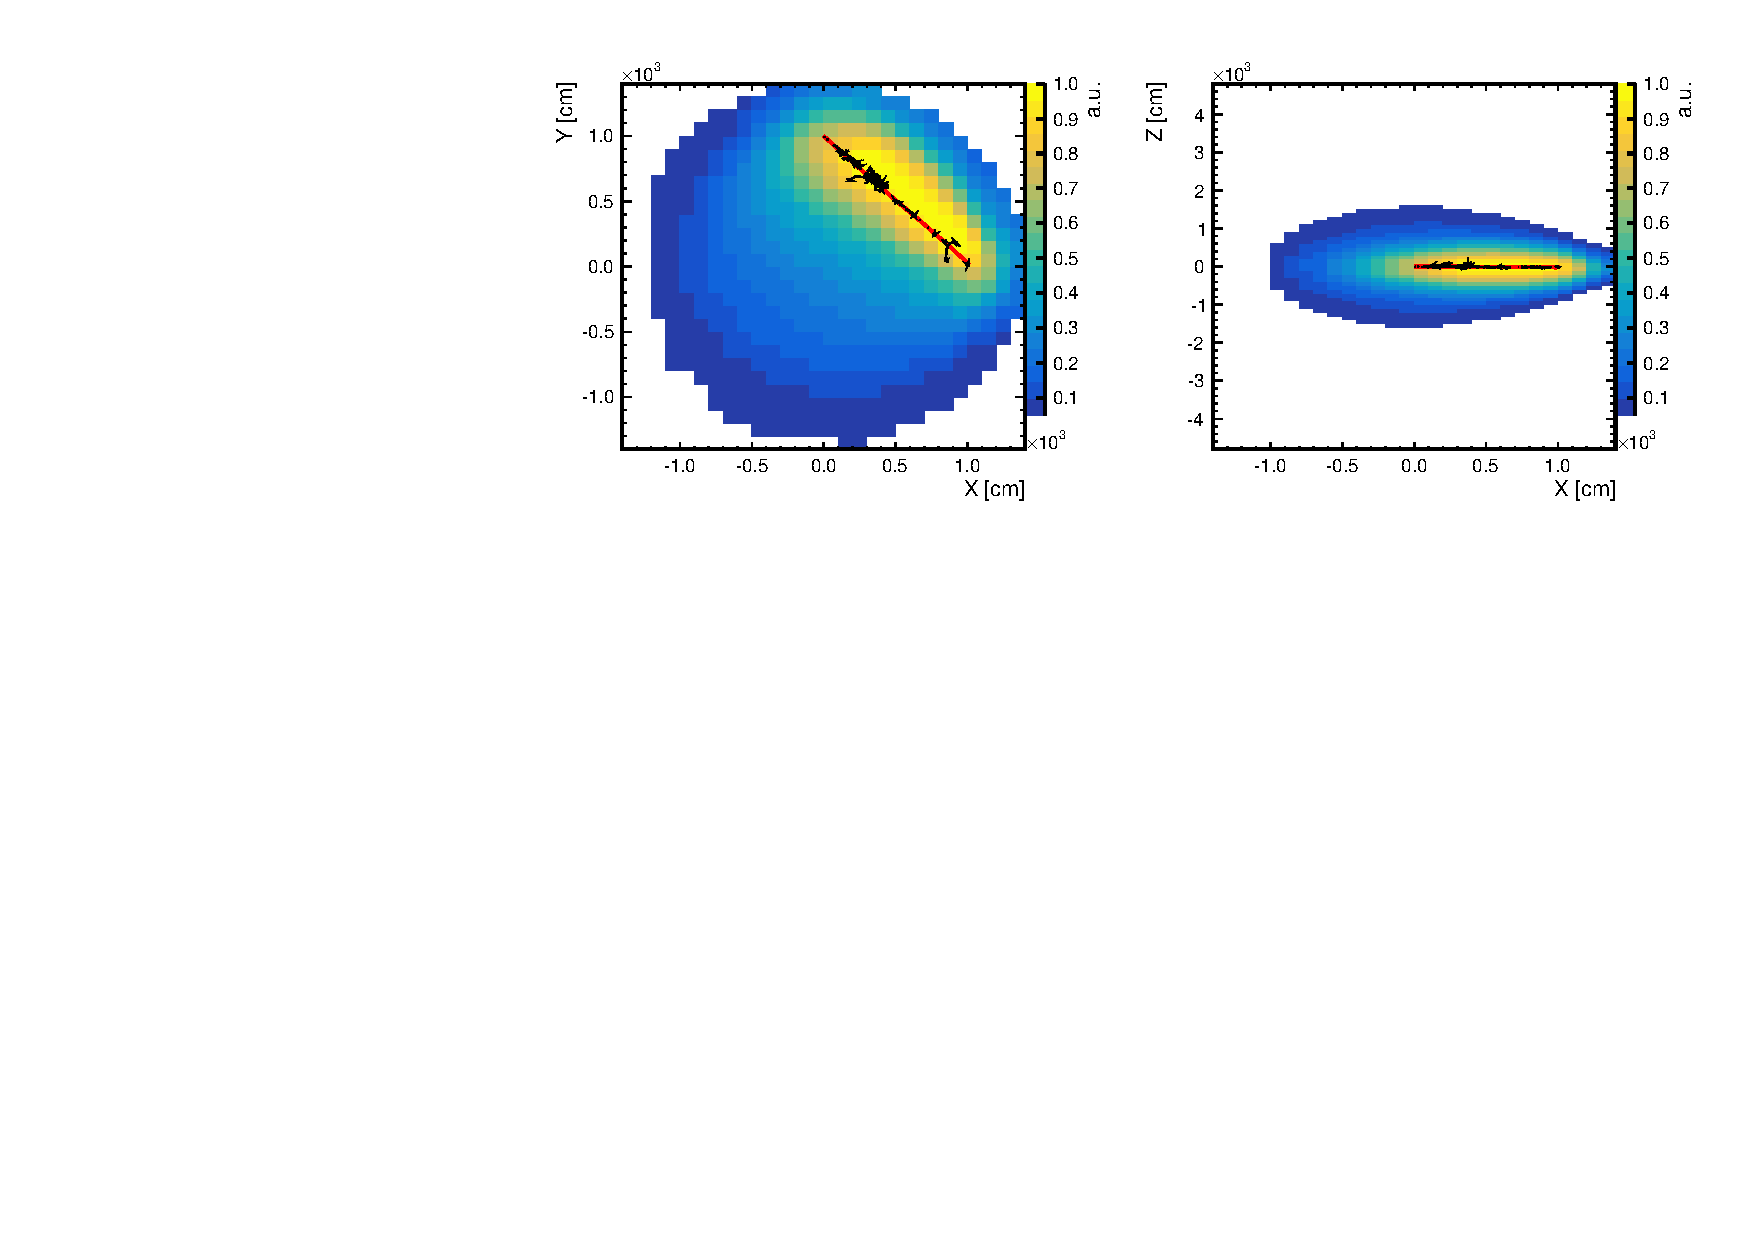
\includegraphics[trim=0.1cm 0.1cm 0.0cm 0.1cm,clip=true,width=\textwidth]
      {./recon/RecoResult0.pdf}
  \end{subfigure}
  ~
    \begin{subfigure}[t]{0.99\textwidth}     
    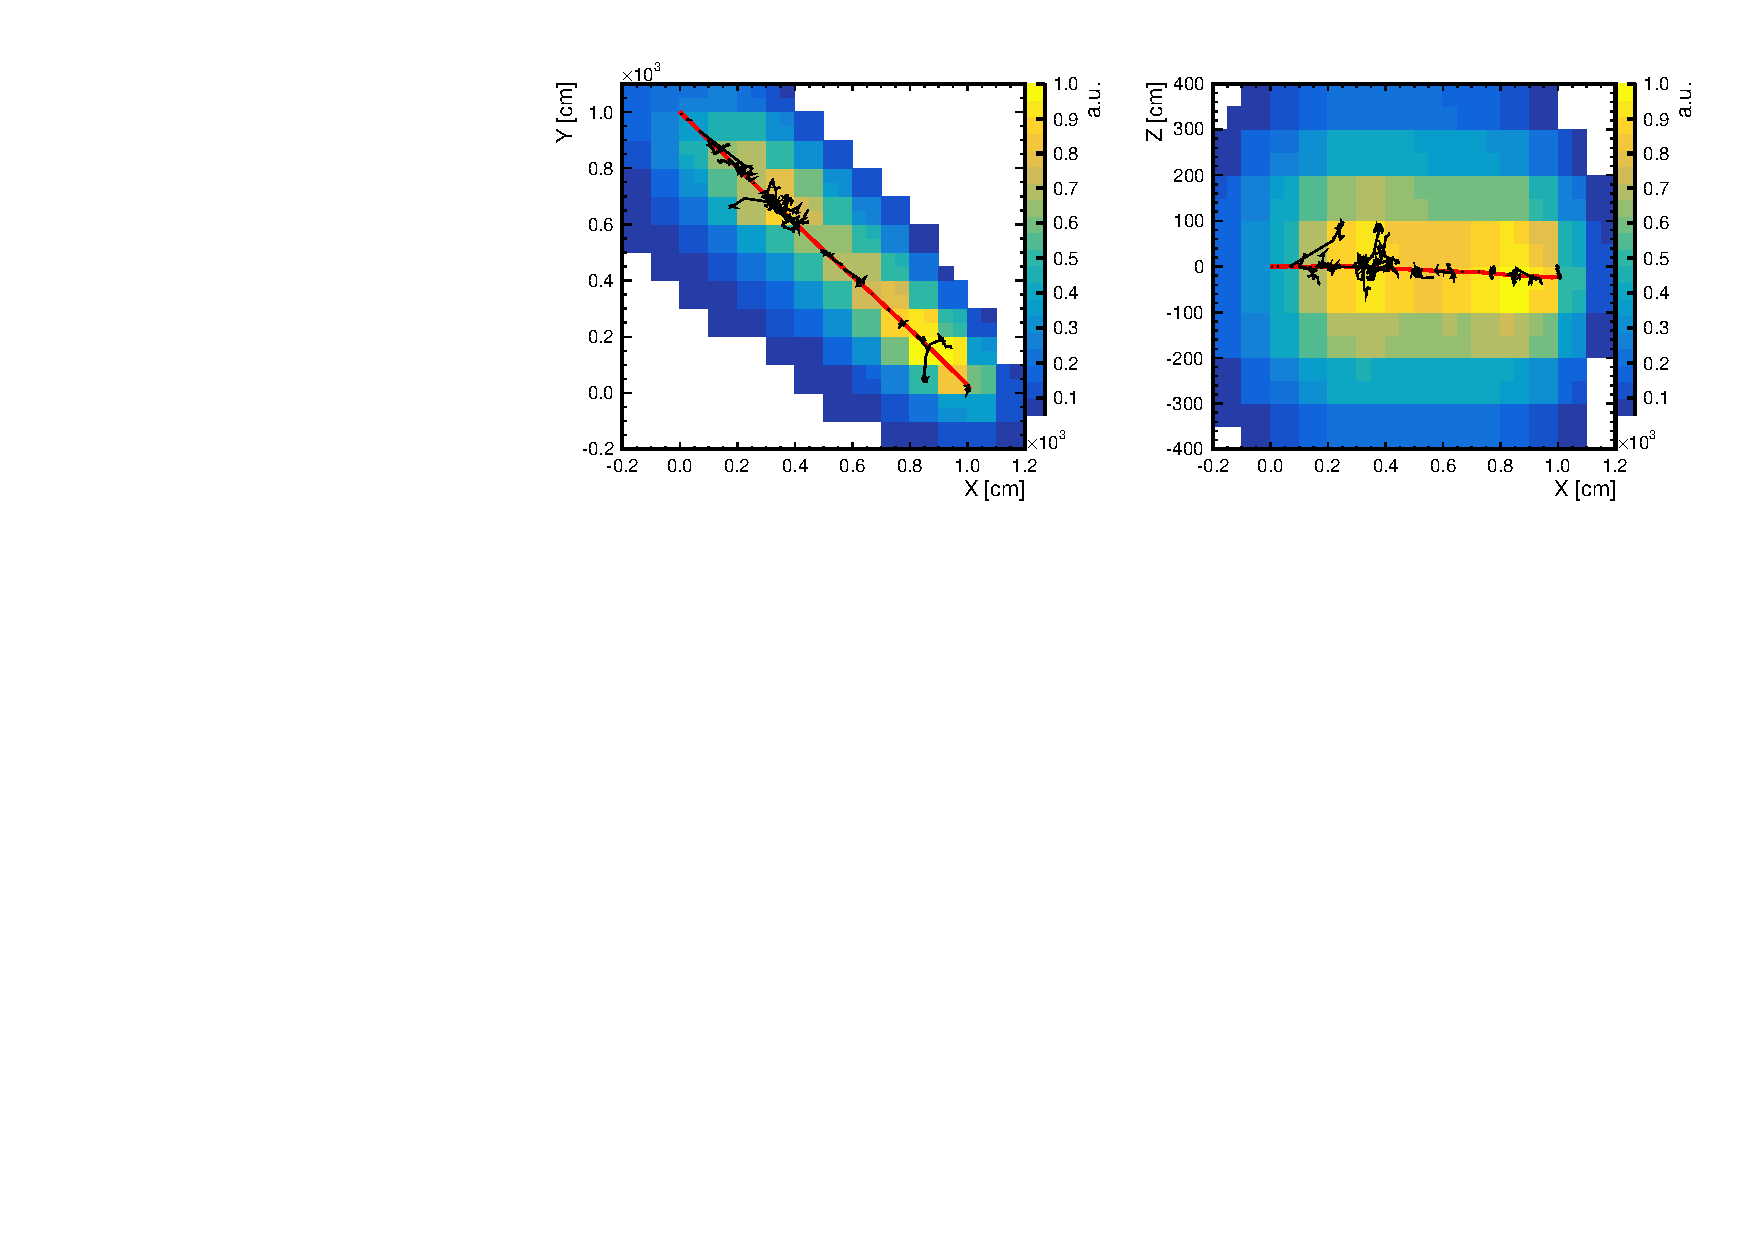
\includegraphics[trim=0.1cm 0.1cm 0.0cm 0.1cm,clip=true,width=\textwidth]
      {./recon/RecoResult8.pdf}
  \end{subfigure}
  ~
  \begin{subfigure}[t]{0.99\textwidth}
    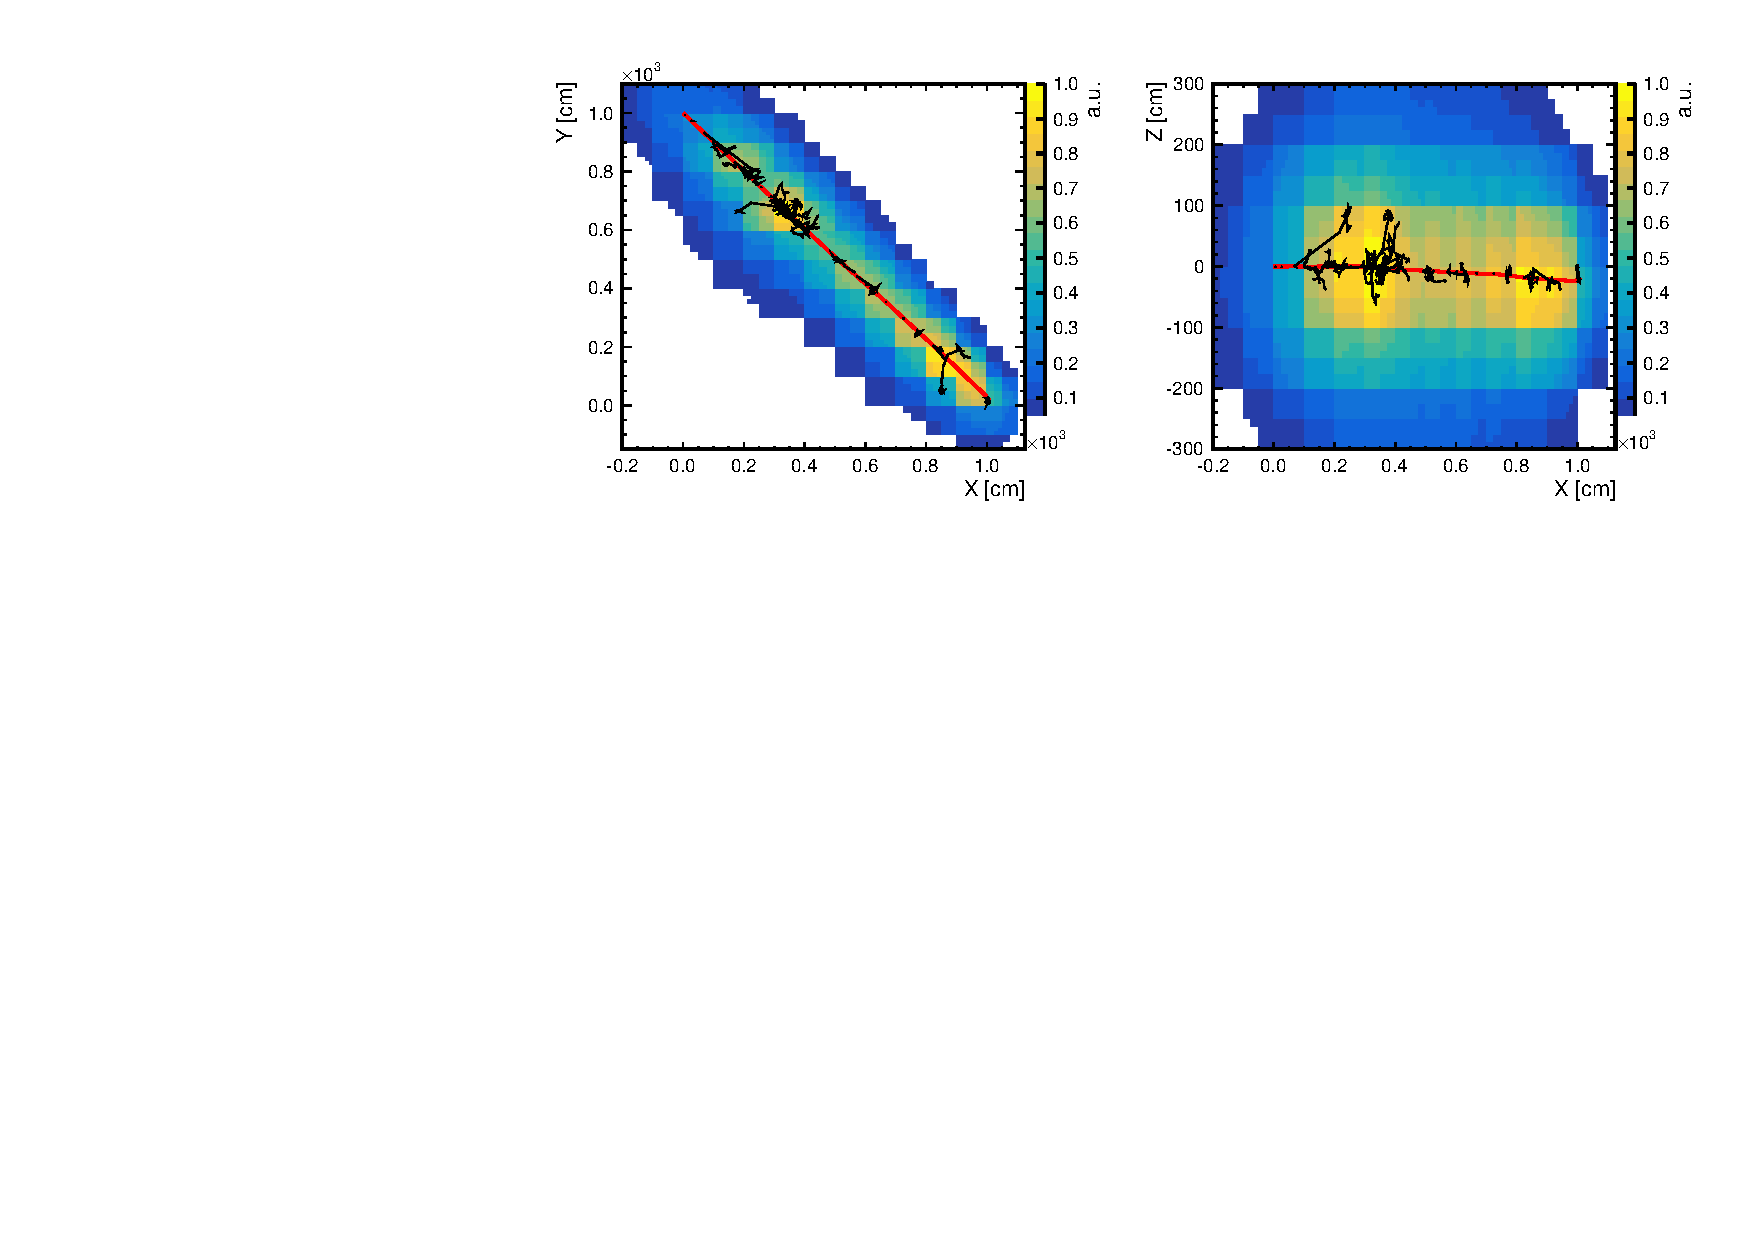
\includegraphics[trim=0.1cm 0.1cm 0.0cm 0.1cm,clip=true,width=\textwidth]
      {./recon/RecoResult21.pdf}
  \end{subfigure}
  \caption{Reconstruction results after the iterations 0 (top), 8 (middle) and 21 (bottom) for a 
simulated muon with $3$\unit{GeV} initial kinetic energy in the cylindrical LENA detector projected 
along the symmetry axis (left) or a radial $y$-axis (right). The primary particle started at 
$(0,\,1000,\,0)$\unit{cm} in the direction $(1,\, -1,\, 0)$. Both the projected tracks of the 
primary particle (red) and of secondary particles (black) are shown. Note that both the axis scales 
and the sizes of the cells change due to the selection of a region of interest and the refinement 
of the reconstruction mesh. Moreover, the cell content is given in a.u. and rescaled such that the 
maximum content is $1$. Some details on the actual reconstruction procedure are given in
\secref{sec:Reconstruction}.
}
  \label{fig:RecoItrResults}
\end{figure}
% ---------- FIGURE END ----------%
  
 % \subsection*{Short summary}
  
 % The whole procedure can be put into this logical sequence:
  
 % \begin{enumerate}
 %  \item Get a reference point
 %  \item Calculate drop-like surface for each signal
 %  \item Smear the surface with the time profile of the signals
 %  \item Add light distribution effects
 %  \item Normalise the probability density distribution for each signal 
 %  \item Use the spatial-dependent light detection efficiency to go from detected light to emitted light
 %  \item Use the result of emitted light as a probability mask and repeat everything starting from point 5
 % \end{enumerate}

 % Since the probability mask will only start to affect everything during the normalisation of the single photon probability density distributions,
 % the iteration can in principle begin at point 5 of this sequence. However, this is very memory intensive, since the raw results of each PMT have
 % to be saved. Thus we choose to begin the iteration loop at point 2. 

 
 
 %technical realisation
  
  \paragraph{Results}
  
  So far this method has mainly been studied with the help of the LENA simulation. This simulation includes only an effective optical model and 
  no Cherenkov light. Furthermore, it was assumed that every photon could be registered separatly. LENA has a coverage of ~30\% resulting in 
  approximatly 250 detected photons per MeV. To reduce the computation time for the reconstruction an adaptive mesh was used. This allowed to 
  establish a voxel size of 12.5 cm in the final iteration. More details about the simulation and the technical implementation of the topological
  reconstruction can be found in \cite{Wonsak:2018uby}.
  
  To proof the robustness and show the potential of this method a large sample of fully contained muons with energies between 1 and 10 GeV was 
  used. An angular resolution between 1.4° at 1~GeV and 0.4° at 10~GeV could be achieved. In addition, the method has been implemented for the JUNO \cite{An:2015jdp}
  detector. First results indicate a high potential for the separation of perfectly point-like events (electrons) from almost point-like events 
  (positrons and gammas) at energies of a few MeV (compare \cite{bwon18}).
  
\paragraph{Application to Cherenkov light}
  
  Some modifications are needed for the application of this method to Cherenkov light. The most obvious one is the 
  time profile $F(t)$, since the Cherenkov process emits the light instantaneously. Thus in most scenarios the timing profile of the photosensors will be the dominant
  factor, which can often be described by a Gaussian with the corresponding time resolution. However, chromatic 
  dispersion of the Cherenkov light must be taken into account if sensors with very good time resolution 
  (below 1 ns) are employed in detectors of the size of THEIA. 
  
  In addition the position dependent detection efficiencies also become direction dependent now, since the Cherenkov 
  light is emitted only in a cone with respect to the particle direction. How to generate such direction dependent
  detection efficiencies is shown for example in \cite{patt09}. However, in general they differ for different particles
  due to the different behaviour when passing through matter. To avoid
  this, we start instead with the basic method without any light distribution effect (detection efficiencies). Thanks to 
  the good timing quality of the Cherenkov-light this already allows to define an accurate volume of interest. In principle,
  this toplogy can then be used for the descion on the direction dependent detection efficiencies. However, this still has to be demonstrated.
  
  %-> Probability to be Cherenkov!
  
 % This is then working well if the method without the iteration process is used. To get reliable results with the whole procedure it is
  

\subsubsection{Low-energy reconstruction} 

by Andrey


%\newpage
%
%% \input{conclusion/outlook.tex}
%
%% BIBLIOGRAPHY
%%__________________________________________________________________________________________________%
%\addcontentsline{toc}{section}{Bibliography}
%\bibliographystyle{unsrt}
%%\bibliography{bib/bibliographyV2}
%\bibliography{RecoBibliography}
%%\bibliography{WonsakBjoern}
%
%
%% DOCUMENT END
%%==================================================================================================%
%\end{document}
%==================================================================================================%